We begin our survey by showing some alarming sybil attacks happening in the
real-world. First, we summarise a few amusing results from external studies,
specifically on the convenience and the scale of the sybil attack. Next, we
describe our experimental study on fake Twitter accounts.

\begin{figure}
  \centering
  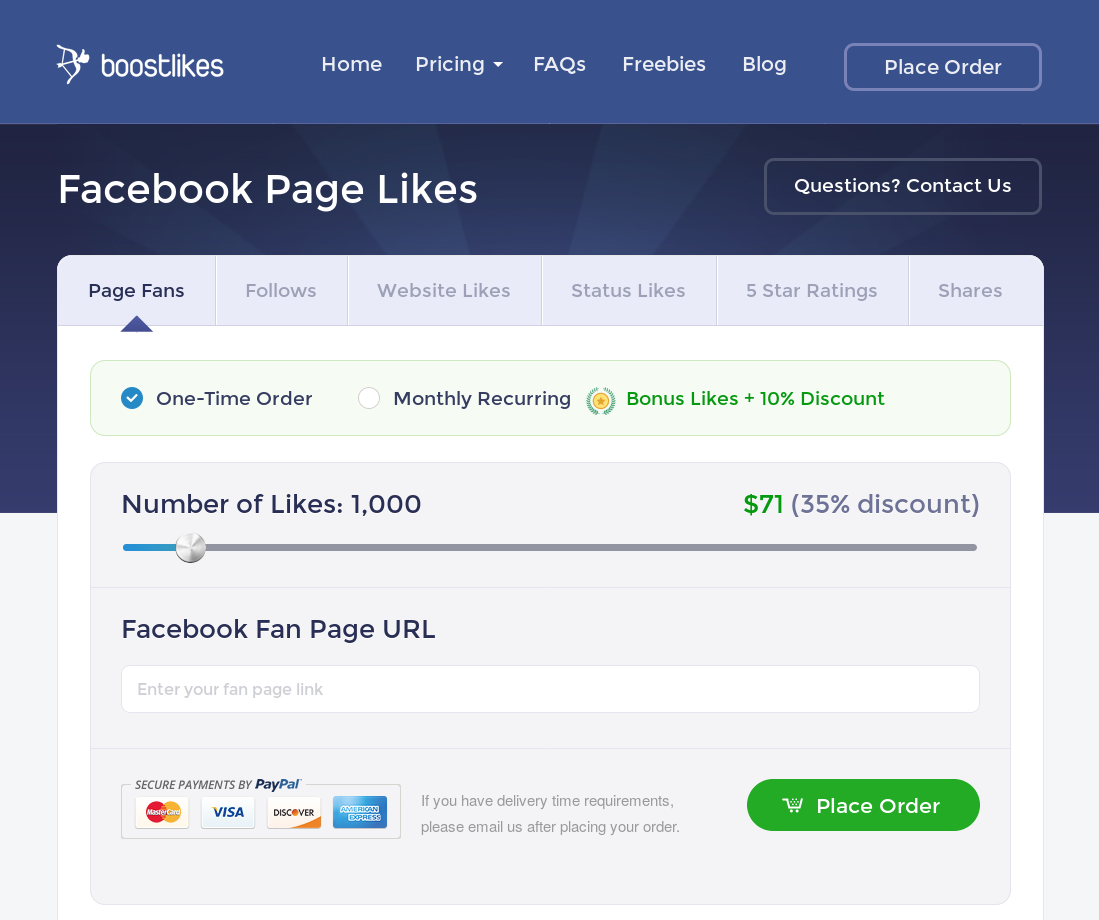
\includegraphics[width=\linewidth]{boostlikes}
  \caption{Screenshot of a commmercial service for buying fake Facebook likes
    called boostlikes.com.}
  \label{fig:boostlikes}
\end{figure}

\begin{figure*}
  \centering
  
\includegraphics[width=\textwidth]{socialformulae}
  \caption{Screenshot of the main banner on socialformulae.com.}
  \label{fig:socialformulae}
\end{figure*}

\subsection{External Studies}
\label{sec:external-studies}

In the introduction we showed how Twitter is used to manipulate public opinion
in elections. But this capability is not only accessible to campaigners with a
large budget. There are marketplaces where anybody can purchase false reputation
scores such as Twitter followers. BoostLikes shown in~\autoref{fig:boostlikes}
is a professionally presented website, it offers a large range of services
including Facebook likes, Twitter followers, Instagram followers and YouTube
views. SocialFormulae (\autoref{fig:socialformulae}) is a similar service but at
a much lower price point, one thousand Twitter followers is only \$9.99. 
% one thousand likes cost \$71 at the time of writing. 

SadBotTrue and its related website Socialpuncher publishes studies on social
media fraud. Two of their studies are particularly useful for demonstrating the
scale of the sybil attack and the obliviousness of Twitter. Firstly, there exist
a sybil group that consist of 3 million accounts. Since their creation, they
generated 2.6 billion tweets. Surprisingly, all the 3 million accounts were
created on the same day---22/10/2013, and the account names are simply numbered
sequentially~\cite{sadbottrue}. Such an obvious activity should be easily
detectable by Twitter, but these accounts are still not closed at the time of
writing. Secondly, the top--100 Twitter users have 523 million unique followers
between them, but 310 million are sybils, that is almost
60\%~\cite{socialpuncher}. Suppose the sybils all belong to the same attacker,
then they can effectively suppress the opinions of the real users.

Clearly, the defence mechanisms employed by popular social network websites are
not adequate to combat the sybil attack. If the sybils infiltrate even more of
our cyberspace, then it may become a form of censorship. Effectively taking away
our right to freedom of speech.

Speaking of censorship, around a million~\cite{tormetric} people use Tor (The
Onion Router)~\cite{dingledine2004tor} to access the uncensored internet when
living in authoritarian regimes such as China, or wish to uphold their privacy
from illegal mass surveillance by intelligence agencies. Unfortunately, Tor
suffered from a sybil attack. In January 2014, 115 bogus relays joined the Tor
network. Six months later, it was discovered that those relays were using a
protocol vulnerability to deanonymise users and find the location of hidden
services. It is unclear to the Tor developers which users are affected or what
information was retrieved, thus it is assumed that users who used Tor between
that period are all affected~\cite{torsybil}. In fact, Tor depends on the fact
that majority of the relays are good to guarantee anonymity with a high
probability. If the network contains a large proportion of sybils, then users
can be easily deanonymised.

\subsection{Small Experiment}
We show it takes less than one hour to obtain over 1000 sybils and investigate
the properties of those sybils. Twitter is selected for two reasons, (1) it is
one of the most popular social networks, (2) it is vulnerabile to the sybil
attack as described in \autoref{sec:external-studies}.

% We crawled Twitter to gain first-hand knowledge on the real-world sybils.
% Twitter was selected because it has an easy-to-use API and it is one of the
% major targets of sybils as mentioned at the top of this section.

\subsubsection{Buying Experience}
Before we can purchase sybils, we needed our own accounts. One was created on
the 25th of November 2016. We made sure our account has 0 tweets and is not
advertised in any other medium over the duration of this experiment. This
guarantees that all of its followers are sybils.

We purchased the ``1,000 Followers'' product from
CoinCrack\footnote{\texttt{https://coincrack.com/}} for \$9. No information was
asked except for an email address for them to deliver the receipt. Followers
started coming in almost immediately after we made our purchase. This is
especially interesting because we made the purchase using Bitcoin, but CoinCrack
did not wait for 10 minutes for our transaction to be confirmed. No more than 1
hour later, our fresh account with 0 tweets has accumulated 1,300 followers.
These followers are sybils, because CoinCrack's website states ``We broker
followers in real time from dozens of engineers across the globe who specilize
in creating/maintaining large amounts of Twitter profiles''.

\subsubsection{Sybil Properties}
Sybils themselves often form relationships in order to emulate real users. To
find these relationships, we crawled our followers recursively for 72 hours
using
\verb!tweetf0rm!\footnote{\texttt{https://github.com/bianjiang/tweetf0rm}}. We
obtained 3 million nodes and 6 million edges at the end of the crawl. Every node
represents an account and every edge represents a ``following'' relationship.
For example, if $A$ follows $B$ then $A$ has a directed edge to $B$. It is
unlikely that all 3 million nodes are sybils. A reasonable assumption is that
real users are unlikely to follow fake accounts because they do not create
interesting or original content. Thus in this work we assume the majority of the
3 million accounts are sybils.

Faloutsos et el.~\cite{faloutsos1999power} analysed the internet topology in
1999 using log-log plots where the $x$-axis is the out-degree and the $y$-axis
is the frequency. We use the a similar methodology to analyse the Twitter graph.
The result is shown in \autoref{fig:twitter-outdeg}. The regression line (green)
is in the form of $p(x) = ax^k$, which is a power-law function. To determine the
goodness-of-fit, we compute the coefficient of determination $R^2$. $R^2$ is a
value between 0 and 1, where 0 indicates no correlation and 1 indicates that the
regression line perfectly fits the data. In this case $R^2 = 0.86$, which
indicates that the Twitter graph fits $p(x)$ reasonably well. We can also see
this visually where the frequency is monotonically decreasing with respect to
the out-degree. This is an interesting observation because many other networks
such as the World-Wide Web, biological networks and other social networks also
have the same property~\cite{faloutsos1999power, girvan2002community}. We do not
have a verifiable explination for this property, but we speculate that it is
because the attackers want to avoid detection, so they structure their sybil
group in a way that look like a group of real users.

% transitivity = 1
% we only show a small portion of all the sybils

\begin{figure}
  \centering
  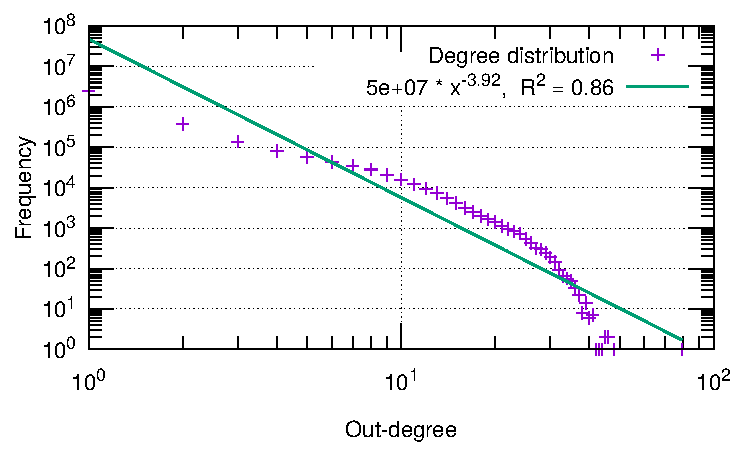
\includegraphics[width=\linewidth]{twitter_outdeg}
  \caption{Graph of out-degree distribution for a graph with 3,248,093 nodes and
    6,062,427 edges.}
  \label{fig:twitter-outdeg}
\end{figure}

%%% Local Variables:
%%% mode: latex
%%% TeX-master: "main"
%%% End:
